%! Author = taj
%! Date = 7/22/25

% Preamble
\documentclass[11pt]{article}

% Packages
\usepackage{amsmath}
\usepackage{graphicx}
\usepackage{float}


\title{Projektna naloga – Termodinamske spremembe}
\author{Taj Šobot, Marcel Maier}

% Document
\begin{document}
    \maketitle
    Projektna naloga pri predmetu Eksperimenti 1.

    \section{Opis naloge}
    Izdelajte preprost eksperimentalni sistem, ki vam omogoča preučevanje izotermnih, izohornih in izobarnih termodinamskih sprememb.
    Izmerite, kako se spreminjajo tlak, prostornina in temperatura plina pri različnih pogojih.
    Pridobljene rezultate predstavite grafično in jih primerjajte s teorijo.

    \section{Eksperimentalna oprema}
    Za ta eksperiment smo sestavili enostavno posodo z batom, ki je na eni strani imela odprtino.
    Vzeli smo dve brizgo (manjša in večja), ki je ponavadi uporabljena za medicinske namene, in ju dali skupaj.
    Velika brizga, ki je služila kot rezervar z zrakom in ima izmerjen notranji volumen:
    \[
        V_v = (75 \pm 2) cm^3
    \]
    Mala brizga pa kot premični bat.
    Ta ima spremenljiv volumen, ki je poljuben od 0 do:
    \[
        V_m = (6.0 \pm 0.2) cm^3.
    \]
    Imamo še en identično brizgo, na katero ni priterjena mala.
    Ta brizga je eksplicitno bila uporabljena pri izotermni spremembi.
    Cevka s katero smo povezala aparat z U cevko ima notranji volumen $V_c = (9 \pm 1) cm^3$
    cevka je bila pri izotermi povezana na tlakometer (od Logger Pro opreme), pri drugih dveh pa na U cevko.
2
    Slika aparatur:
    \begin{figure}[H]
        \centering
        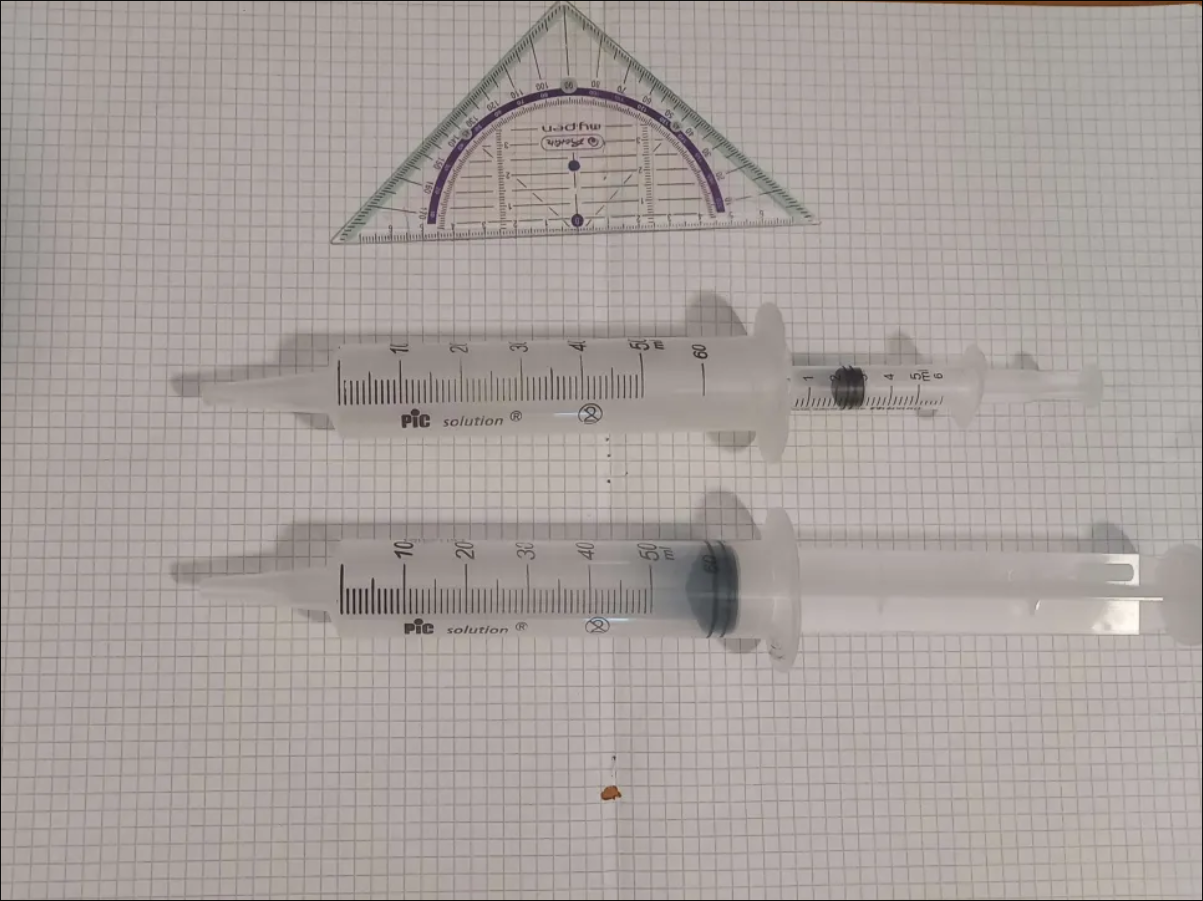
\includegraphics[width=0.7\textwidth]{slika1}
        \caption{Brizge}
        \label{fig:1}
    \end{figure}
    Skica eksperimenta:
    \begin{figure}[H]
        \centering
        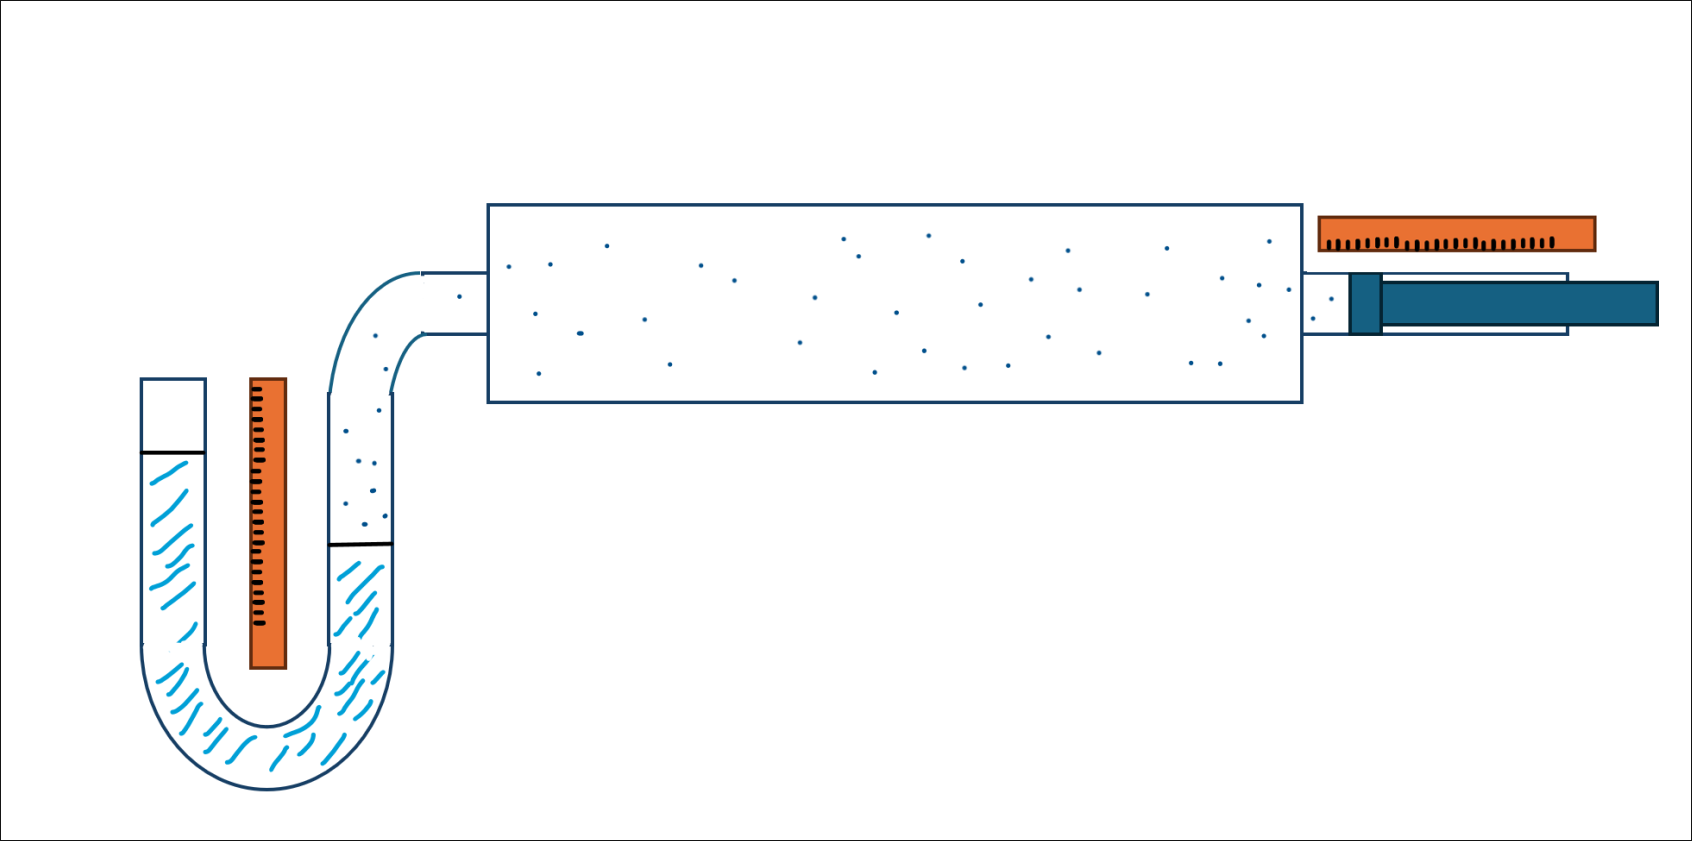
\includegraphics[width=0.7\textwidth]{slika2}
        \caption{Skica}
        \label{fig:1b}
    \end{figure}

    \section{Meritve}
        Na lokaciji merjenja je bil tisti dan zračni tlak
        \[
            p_0 = (101,4 \pm 0,1) kPa
        \]
        Vse enačbe so izpeljane iz enačbe za idealni plin:
        \[
            P V = n R T
        \]
        \subsection{Izoterma}
        Pri tej td. spremembi temperatura ($T[K]$) ostaja konstantna.
        Za to spremembo velja:
        \[
            P_1 V_1 = P_2 V_2 = konst.
        \]
        Zato smo merili, kako se tlak spreminja, ko spreminjamo volumen.
        V spodnji tabeli so naše meritve

        \begin{table}[H]
            \centering
            \begin{tabular}{|c|c|}
                \hline
                \textbf{p [kPa]} & \textbf{$V_v [cm^3]$} \\
                \hline
                105.3  & 45  \\
                113.75 & 40  \\
                123.85 & 35  \\
                135.4  & 30  \\
                150    & 25  \\
                168.8  & 20  \\
                190.6  & 15  \\
                \hline
            \end{tabular}
            \caption{Meritve tlaka in prostornine}
            \label{tab: meritve1}
        \end{table}
        Napake:
        \begin{align*}
            V_v{err} = 1 mc^3 \\
            p_{err} = 0.1 kPa
        \end{align*}
        Opomba: bat smo pri tem delu eksperimanta premikali počasi z pomočjo primeža, tako smo zagotovili minimalno spreminjanje temperature.

        \subsection{Izohora}
        Pri tej td. spremembi volumen ($V[m^3]$) ostaja konstantna.
        Za to spremembo velja:
        \[
            \frac{T_1}{P_1} = \frac{T_2}{P_2} = konst.
        \]
        Zato smo merili, kako se tlak spreminja, ko spreminjamo temperaturo zraka.
        V spodnji tabeli so naše meritve

        \begin{table}[H]
            \centering
            \begin{tabular}{|c|c|c|}
                \hline
                $T[C^\circ]$ & $\Delta h[cm]$ & $\Delta p[Pa]$\\
                \hline
                30 & 5.8  & 570 \\
                35 & 10.2 & 1000 \\
                40 & 15.8 & 1550 \\
                45 & 18.6 & 1820 \\
                50 & 21.6 & 2120 \\
                \hline
            \end{tabular}
            \caption{Meritve temperature in višinske razlike}
            \label{tab:temp-dh}
        \end{table}
    \begin{align*}
        T_{err} = 1 C^{\circ} \\
        h_{err} = 0.1 cm \\
        p_{err} = 50 Pa
    \end{align*}


    \subsection{Izobara}
        Pri tej td. spremembi tlak ($p[Pa]$) ostaja konstantna.
        Za to spremembo velja:
        \[
            \frac{T_1}{V_1} = \frac{T_2}{V_2} = konst.
        \]
        Zato smo merili, kako se spreminja volumen, ko spreminjamo temperaturo zraka.
        V spodnji tabeli so naše meritve

    \begin{table}[H]
        \centering
        \begin{tabular}{|c|c|}
            \hline
            \textbf{T [$C^\circ$]} & \textbf{$\Delta V_m$ [cm\textsuperscript{3}]} \\
            \hline
            30                     & 1.2                                           \\
            35                     & 2.3                                           \\
            40                     & 3.2                                           \\
            45                     & 4.8                                           \\
            50                     & 5.8                                           \\
            \hline
        \end{tabular}
        \caption{Volumske spremembe pri različnih temperaturah}
        \label{tab:temp-dV}
        \end{table}

    Napake:
    \begin{align*}
        T_{err} = 1 C^{\circ} \\
        V_m{err} = 0.2 cm^3 \\
    \end{align*}

    \section{Grafi in rezultati}
        \subsection{Izoterma}
        Za izotermo velja:
        \[
            p(V) = n R T\frac{1}{V}
        \]
        Sledi lineariziran graf:
        \begin{figure}[H]
            \centering
            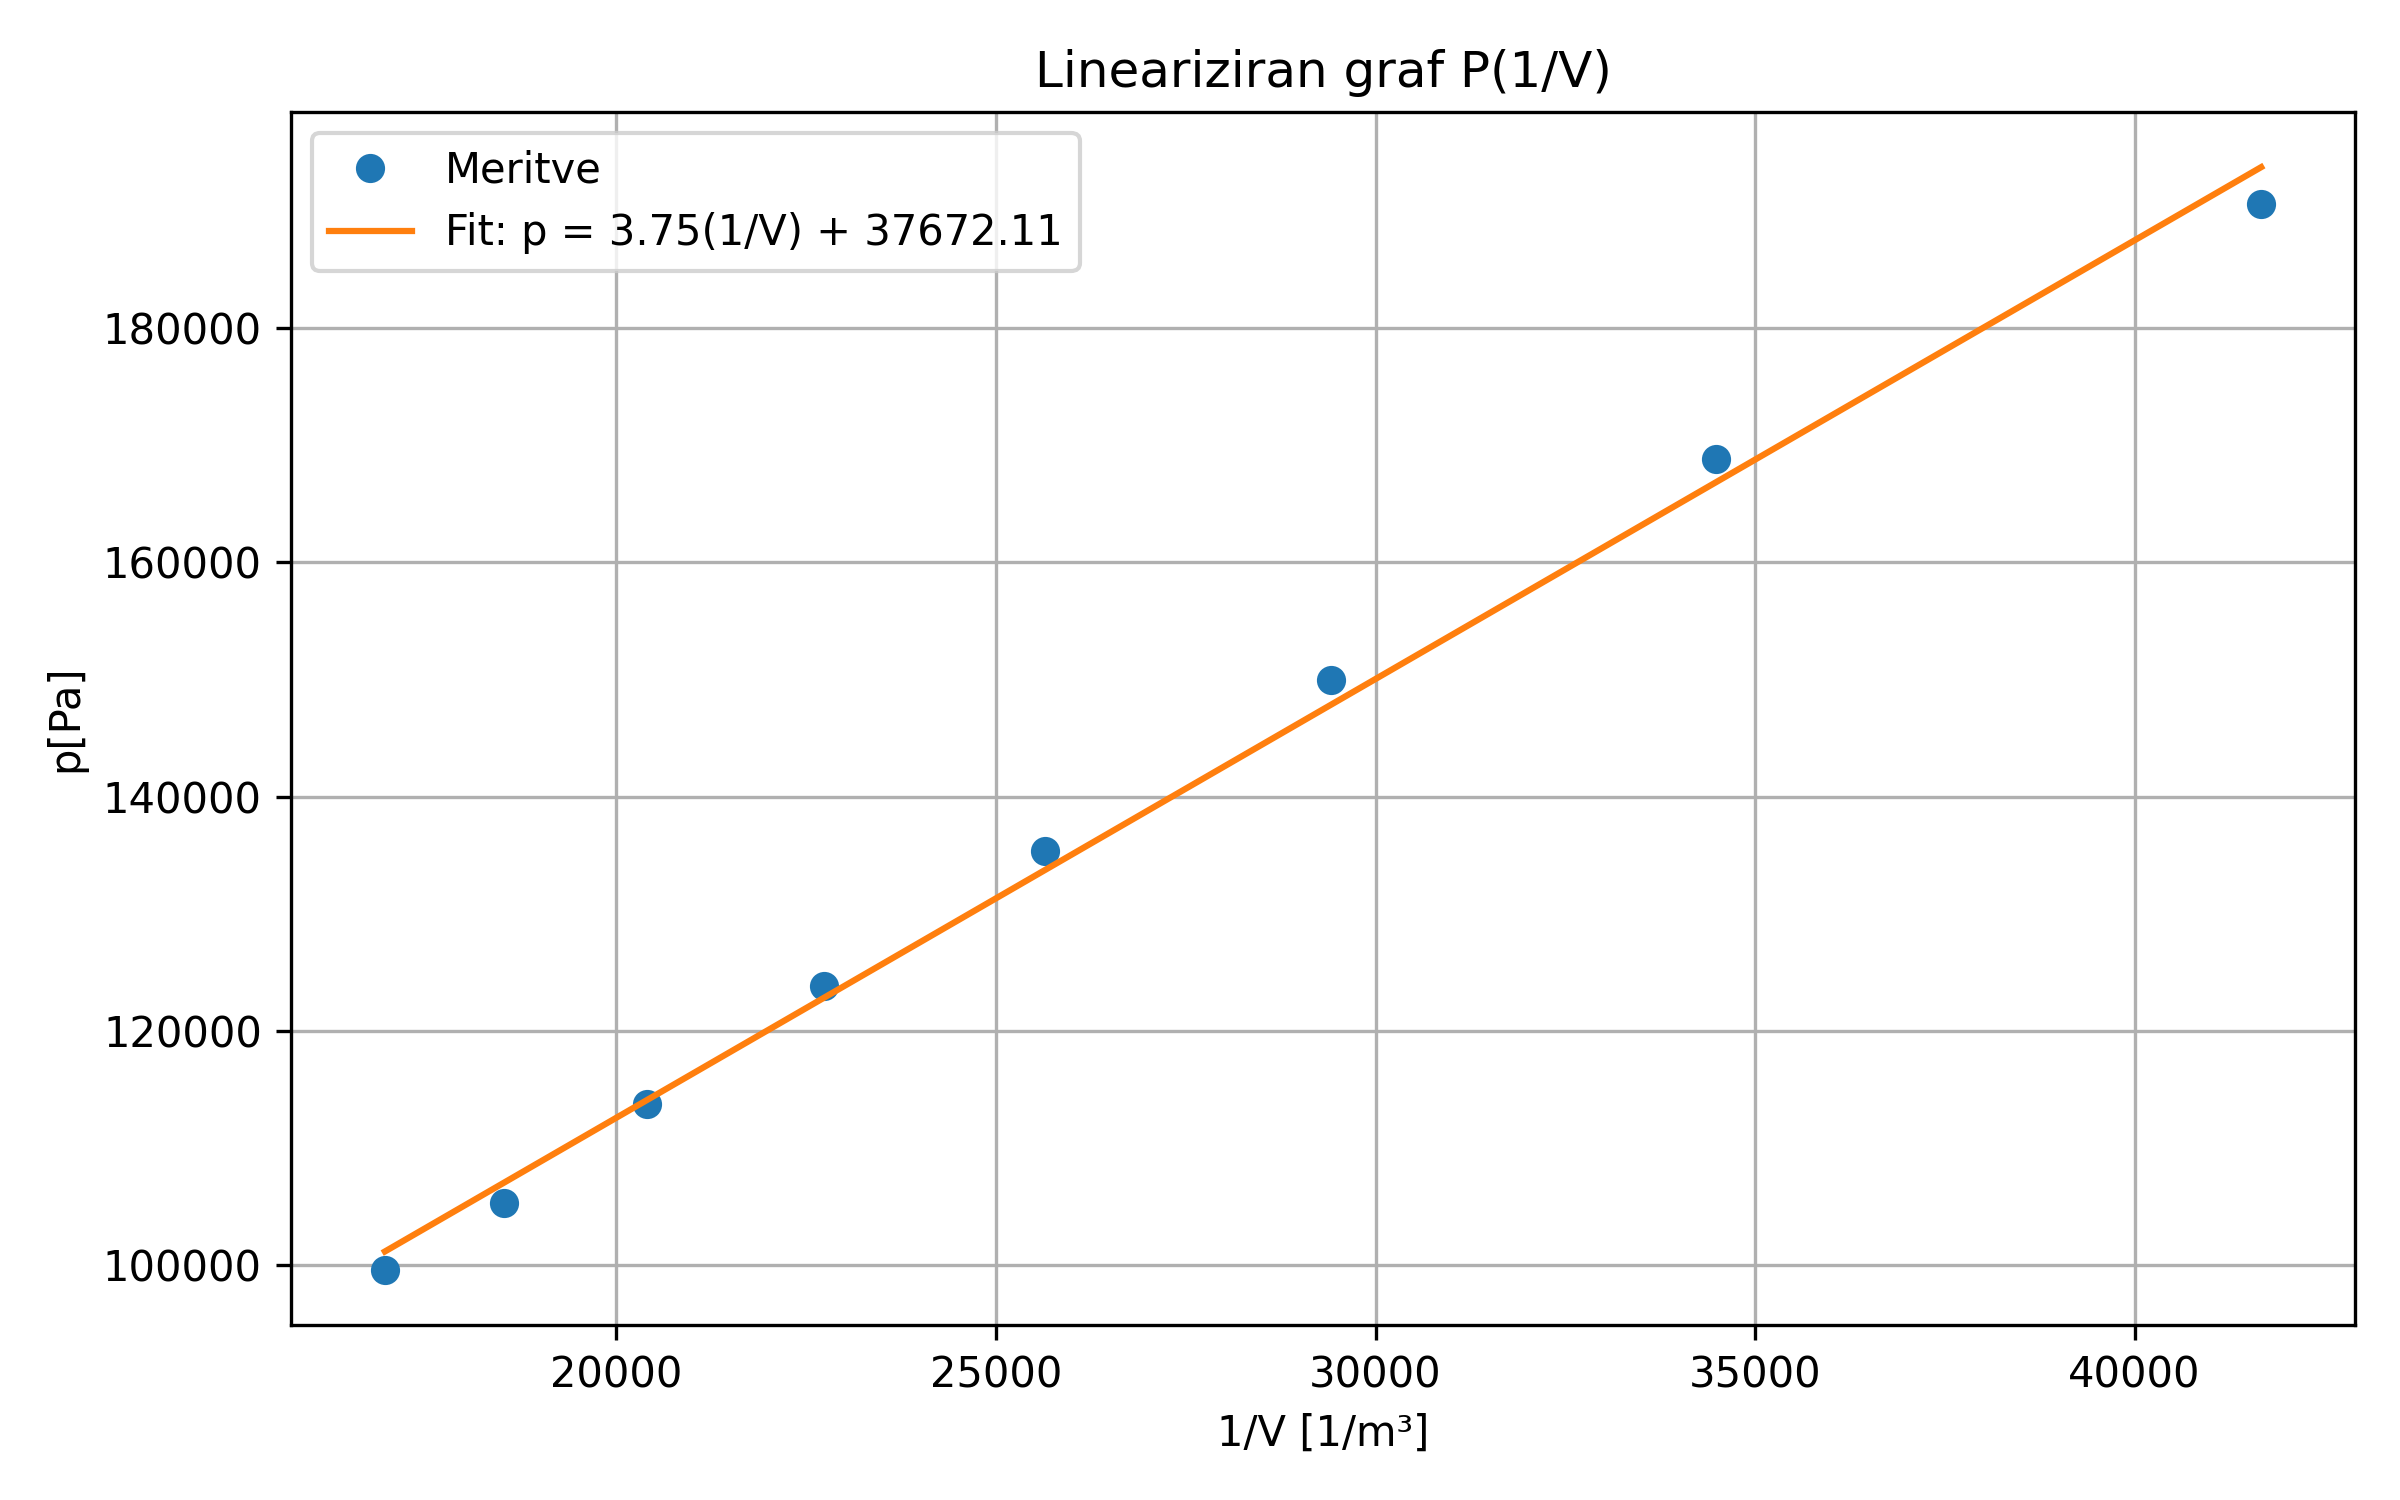
\includegraphics[width=0.7\textwidth]{graf1}
            \caption{Graf p(1/V)}
            \label{fig:2}
        \end{figure}
        Konstantni člen je potem:
        \[
            n R T = 3.75 \pm 0.04
        \]

        \subsection{Izohora}
        Za izobaro velja:
        \[
            p(T) = \frac{n R}{V} T
        \]
        Sledi lineariziran graf:
        \begin{figure}[H]
            \centering
            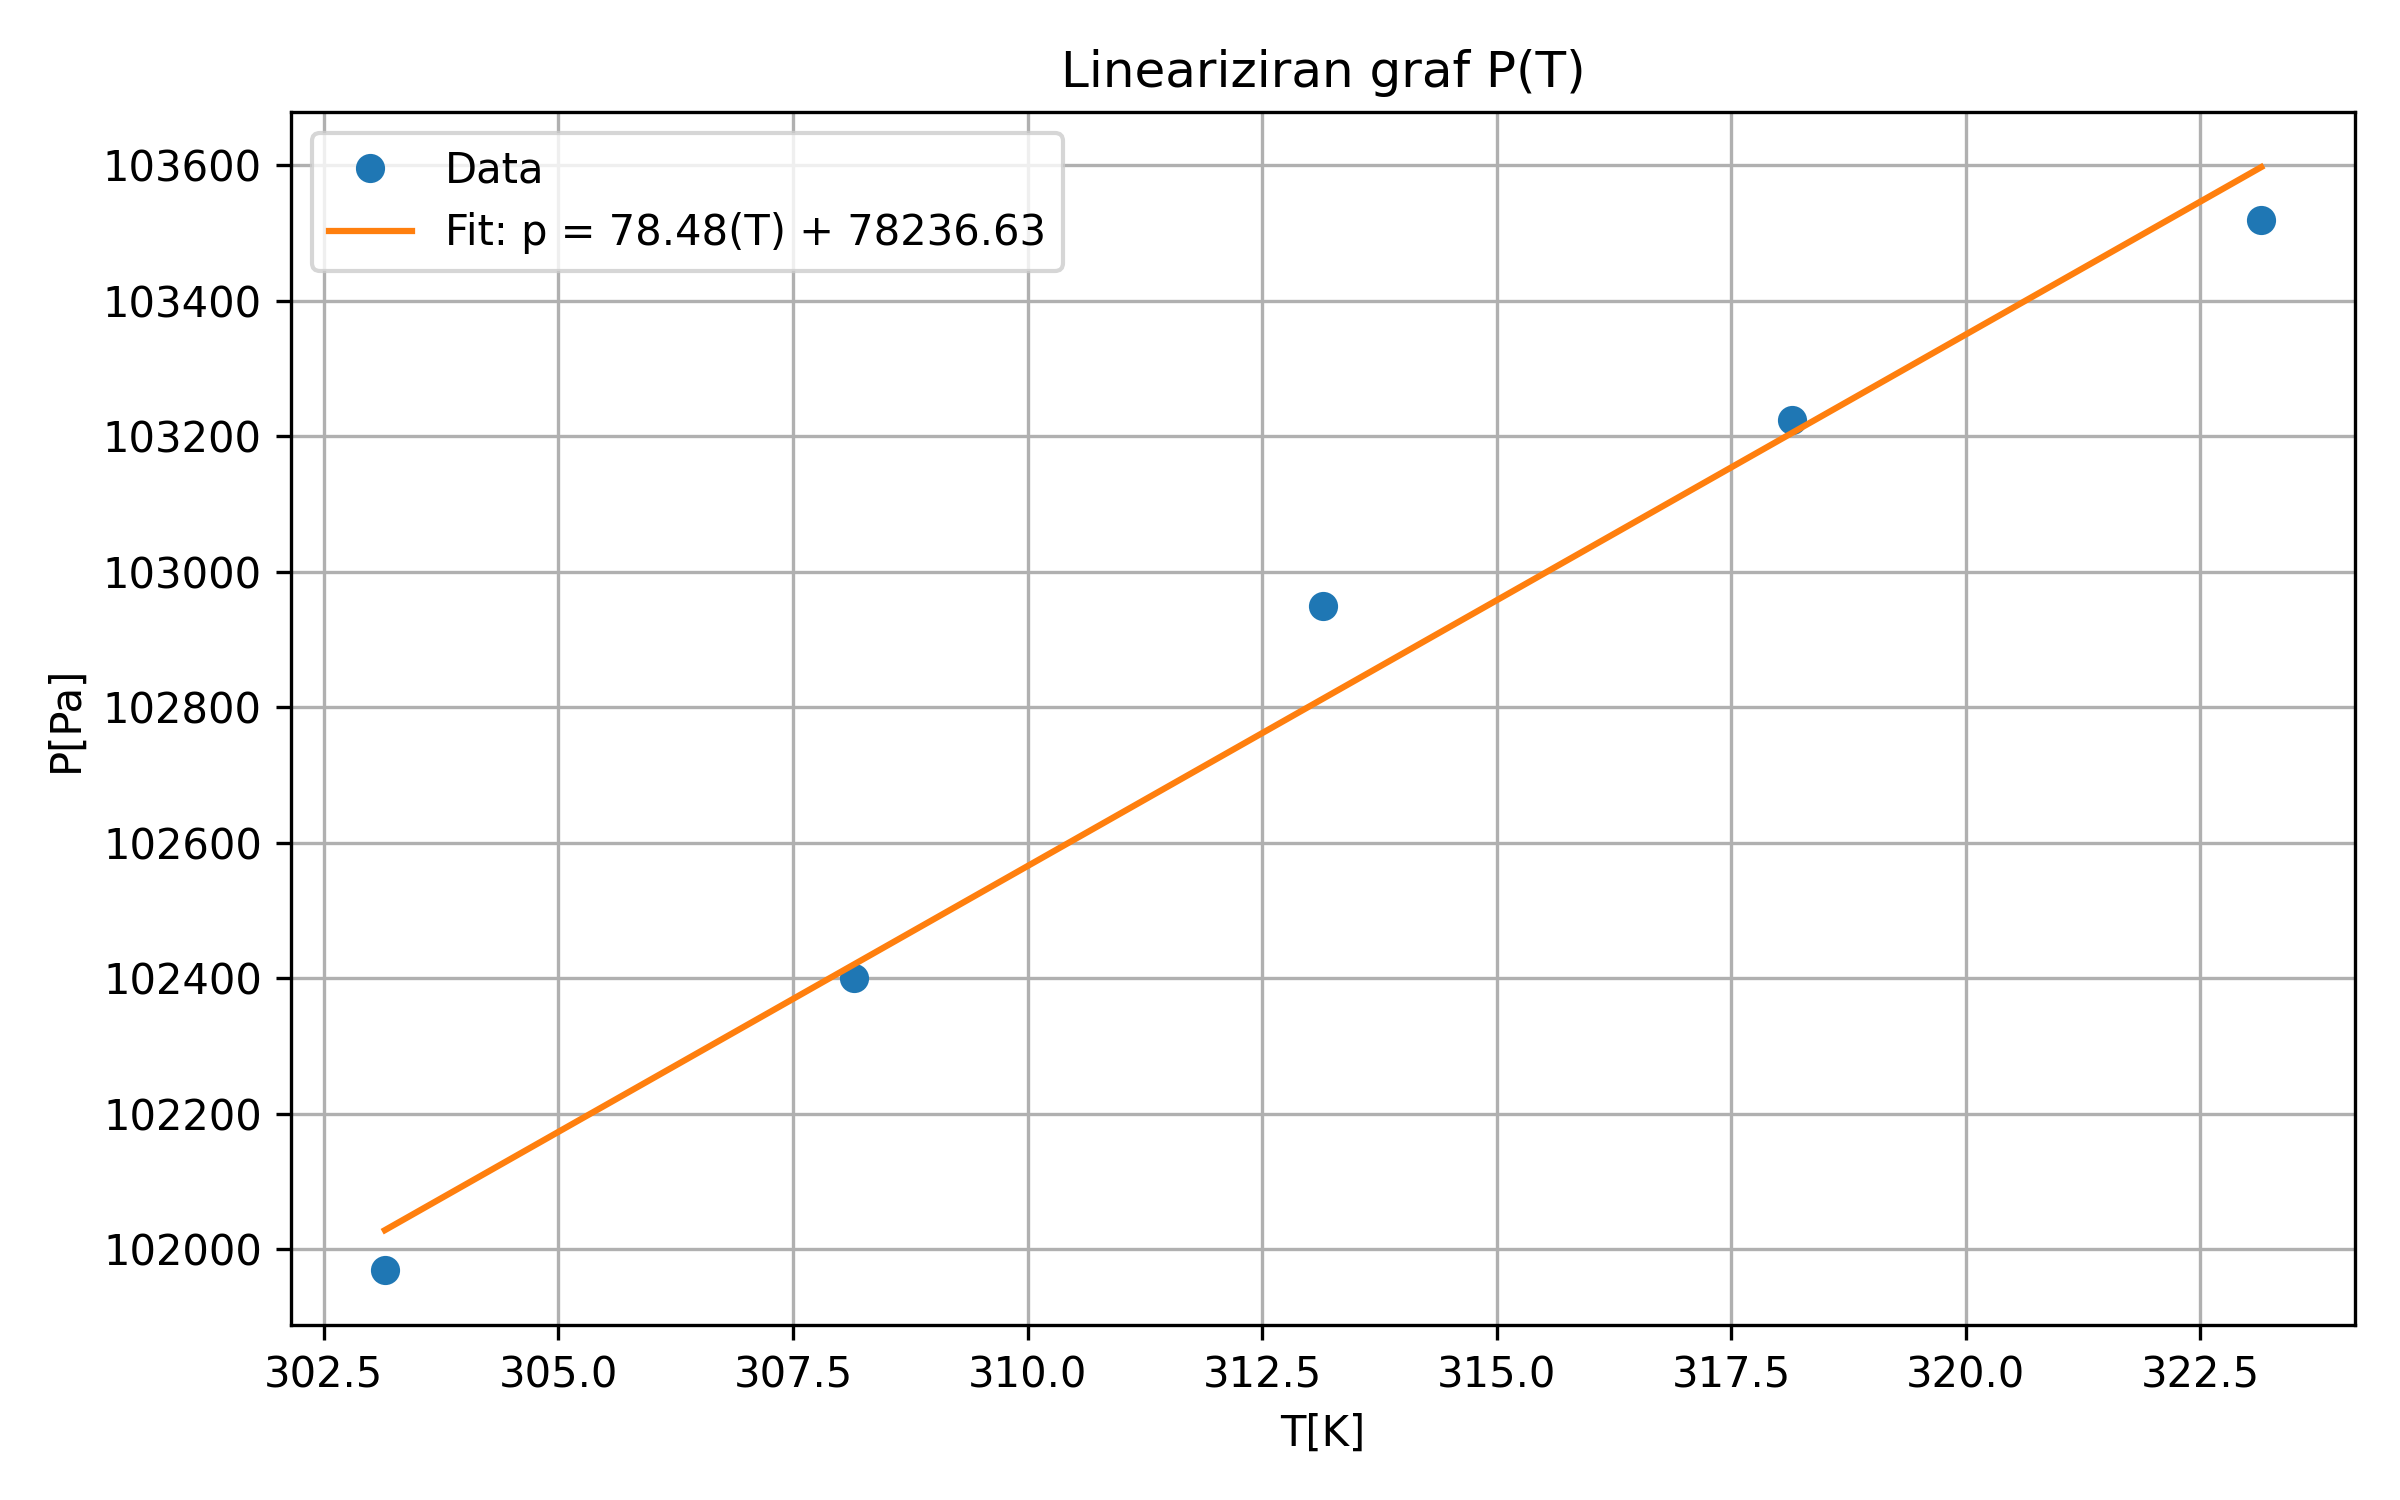
\includegraphics[width=0.7\textwidth]{graf2}
            \caption{Graf p(T)}
            \label{fig:3}
        \end{figure}
        Konstantni člen je potem:
        \[
            \frac{n R}{V} = 78.5 \pm 0.9
        \]

        \subsection{Izobara}
        Za izobaro velja:
        \[
            V(T) = \frac{n R}{p} T
        \]
        Sledi lineariziran graf:
        \begin{figure}[H]
            \centering
            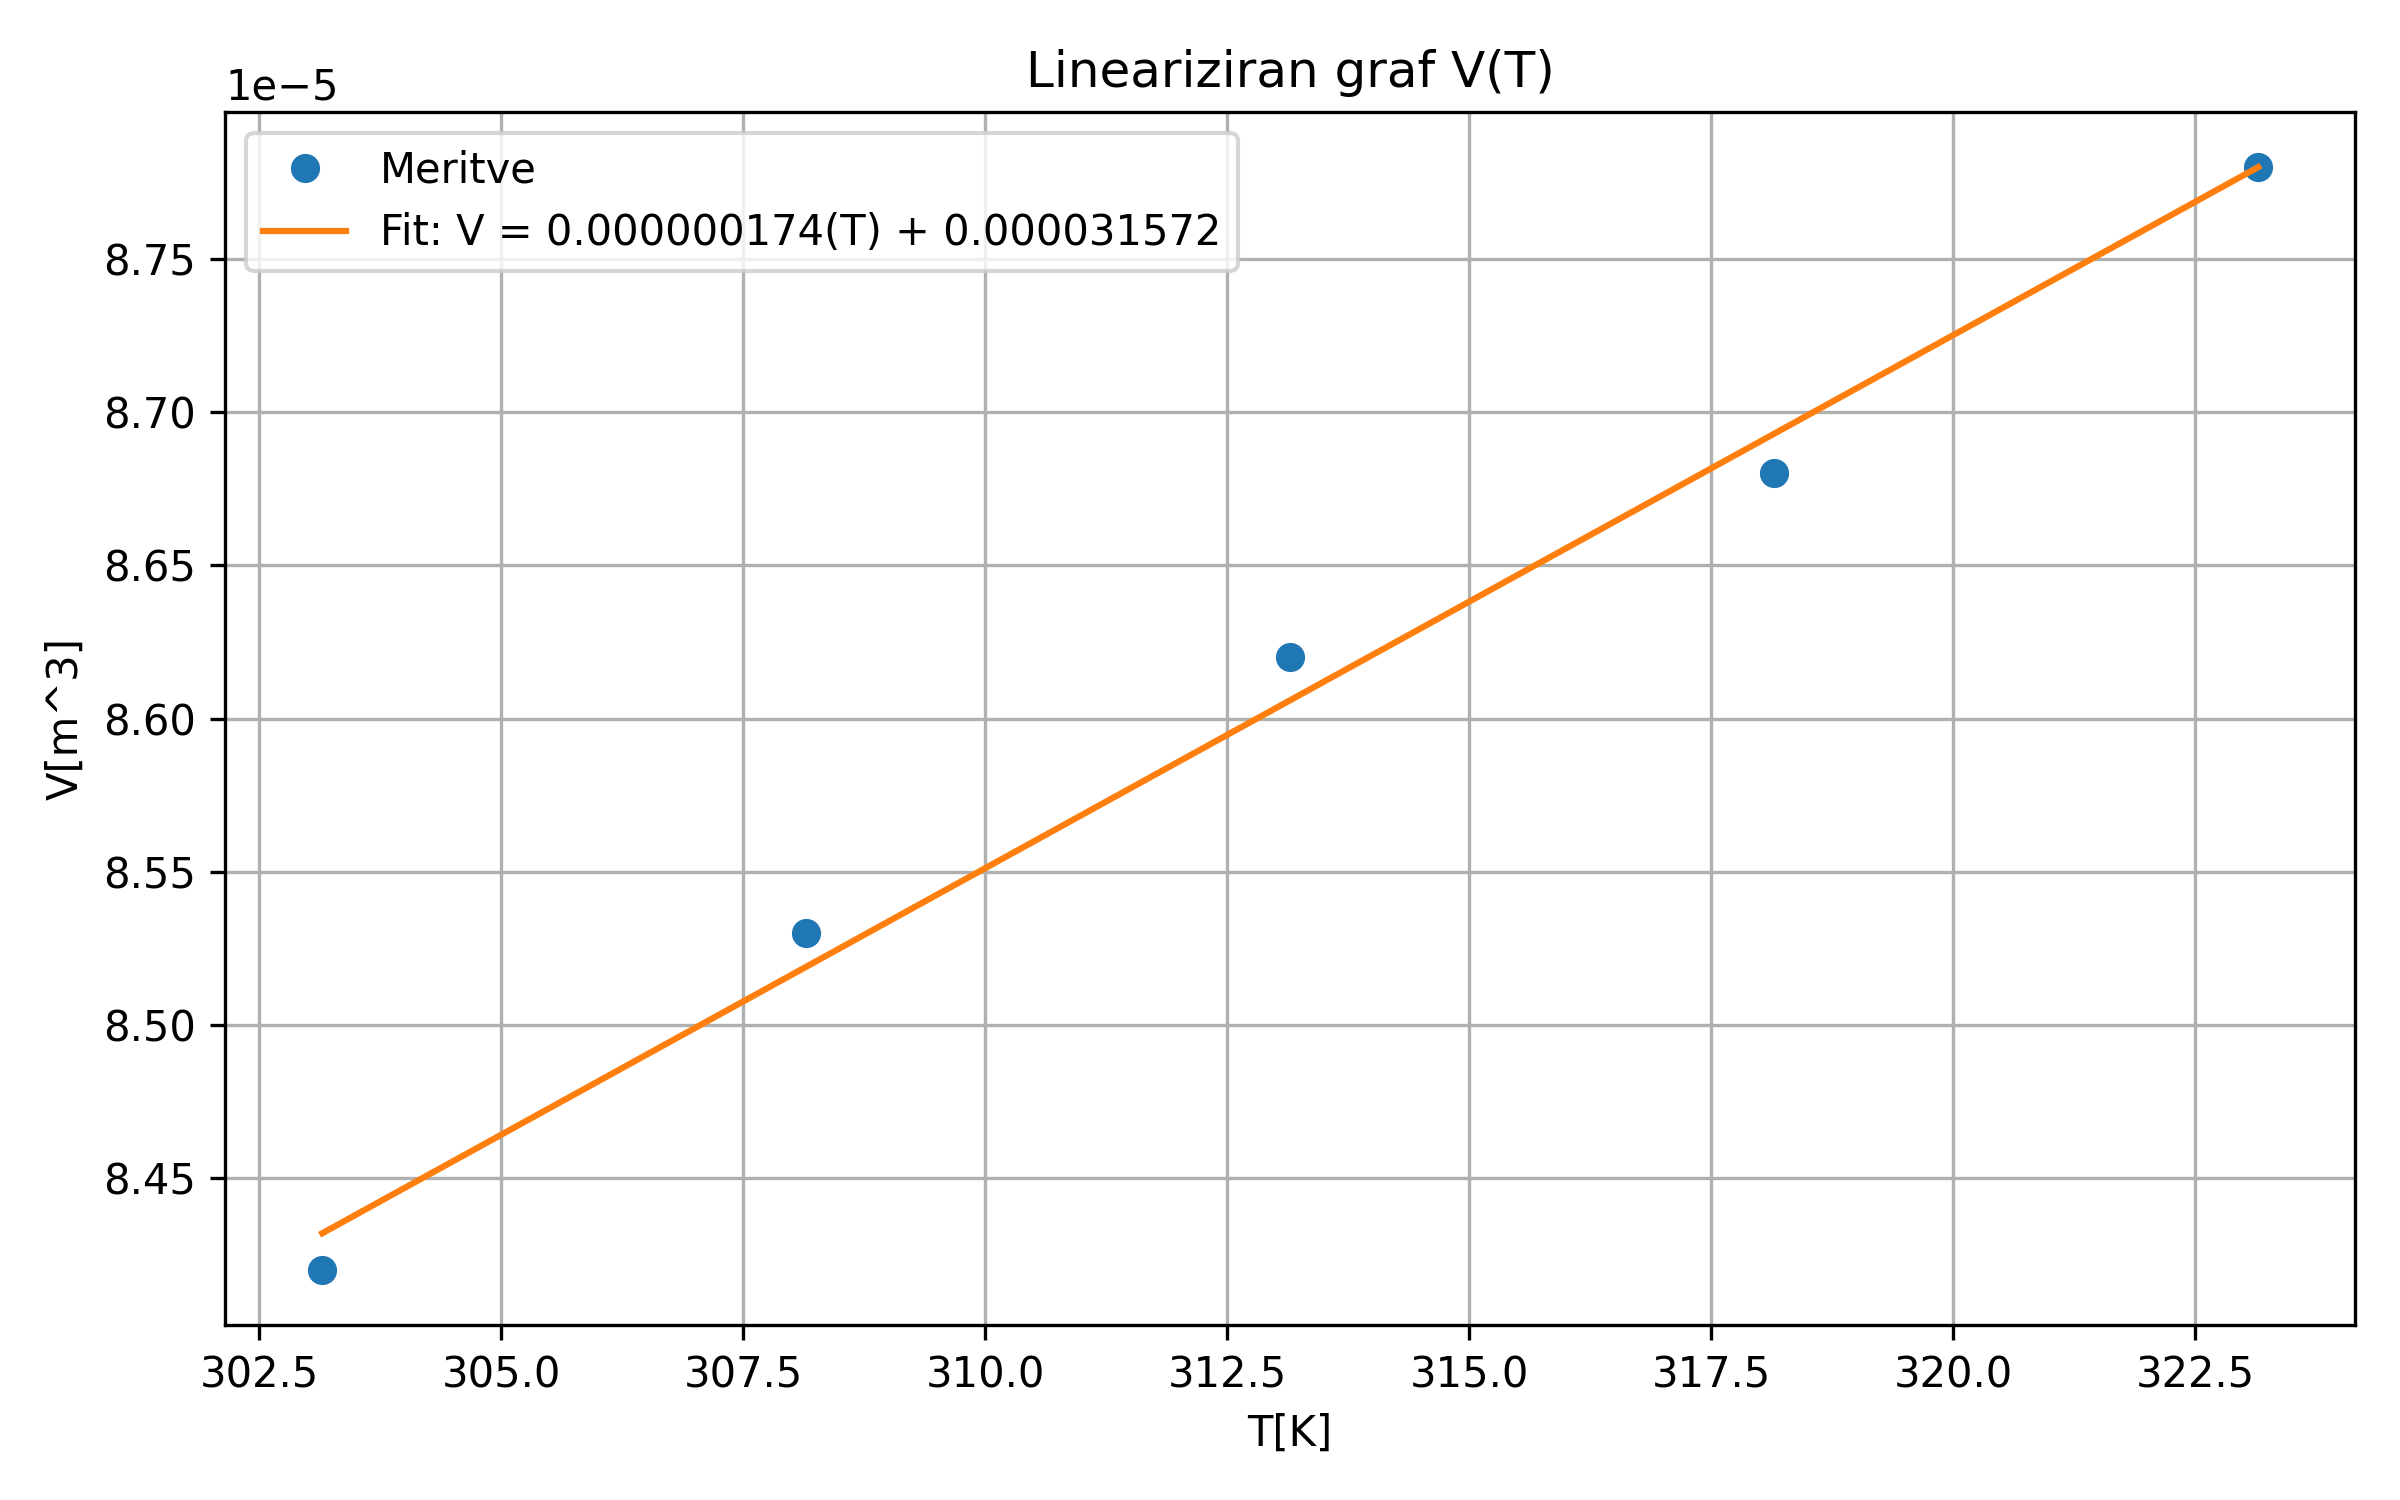
\includegraphics[width=0.7\textwidth]{graf3}
            \caption{Graf V(T)}
            \label{fig:4}
        \end{figure}
        Konstantni člen je potem:
        \[
            \frac{n R}{p} = (1.74 \pm 0.03)*10^{-7}
        \]
    \section{Zaključek}
        Kot smo videli iz grafov se teoretični model strinja z izmerjenimi vrednostmi.
        V eksperimentu smo tudi spoznali, kako lahko vsakdanje pripomočke uporabimo za neko eksperimentalno delo.

\end{document}